
\documentclass{article}

\input{preamble.sty}

\usepackage{hyperref, tikz}
\usetikzlibrary{decorations.pathmorphing}

\begin{document}

  \setcounter{section}{7}
  \section{\sc WAR and Contract Valuation}

    \subsection{\sc Wins above Replacement}

      Wins above Replacement (WAR), baseball's flagship metric, summarizes player performance in a single number. For position players, it starts with batting runs, baserunning runs and fielding runs, which we have already covered. For catchers, fielding runs includes framing runs, blocking runs, and other metrics unique to catchers (challenge runs?). By measuring all of these skills in the same units, we have prepared ourselves to add them together in a meaningful way.

      The diagram below illustrates the FanGraphs pipeline for calculating WAR.

      \begin{center}
        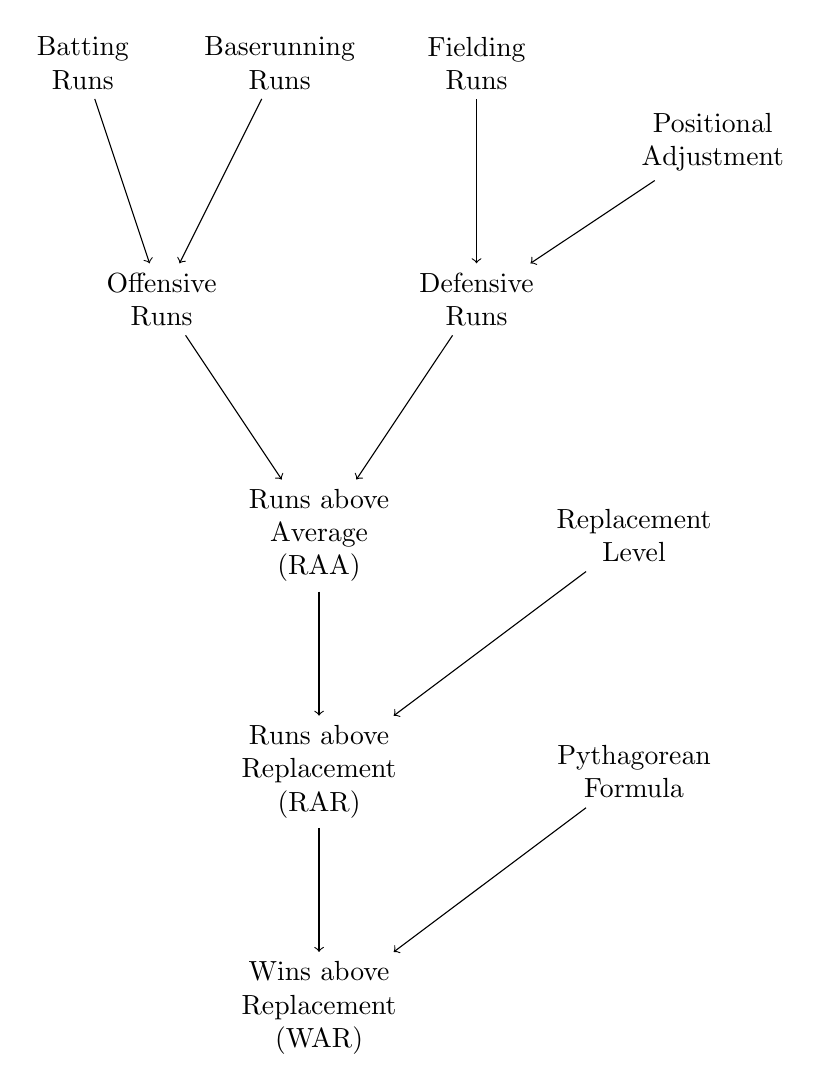
\begin{tikzpicture}
          \node[align=center](bat) at (-3, 12) {Batting \\ Runs};
          \node[align=center](run) at (-0.5, 12) {Baserunning \\ Runs};
          \node[align=center](fld) at (2, 12) {Fielding \\ Runs};
          \node[align=center](pos) at (5, 11) {Positional \\ Adjustment};
          \node[align=center](off) at (-2, 9) {Offensive \\ Runs};
          \node[align=center](def) at (2, 9) {Defensive \\ Runs};
          \node[align=center](replacement) at (4, 6) {Replacement \\ Level};
          \node[align=center](raa) at (0, 6) {Runs above \\ Average \\ (RAA)};
          \node[align=center](pythag) at (4, 3) {Pythagorean \\ Formula};
          \node[align=center](rar) at (0, 3) {Runs above \\ Replacement \\ (RAR)};
          \node[align=center](war) at (0, 0) {Wins above \\ Replacement \\ (WAR)};
          \draw[->] (bat) -- (off);
          \draw[->] (run) -- (off);
          \draw[->] (fld) -- (def);
          \draw[->] (pos) -- (def);
          \draw[->] (off) -- (raa);
          \draw[->] (def) -- (raa);
          \draw[->] (raa) -- (rar);
          \draw[->] (replacement) -- (rar);
          \draw[->] (rar) -- (war);
          \draw[->] (pythag) -- (war);
        \end{tikzpicture}
      \end{center}

      \subsubsection{\sc Positional Adjustment}

        We don't use fielding runs directly in runs above average (RAA) because of how it is defined. Fielding runs evaluates a player relative to an average player at the same position, but an average shortstop is not the same as an average first baseman. Teams put their best defensive players at shortstop because of the demands of the position, and they often hide their worst defenders at first base. We don't want to place the same value on average shortstop play as we do on average first base play.

        Enter positional adjustments. The idea behind positional adjustments is to add a number to a player's fielding runs to account for the difficulty of their position to make apples-to-apples comparisons between, for example, shortstop and first base. There is an ongoing debate between two approaches to positional adjustment: offense-based adjustments and defense-based adjustments.

        Offense-based positional adjustments are based on the idea of comparing the scarcity of average defensive skill between positions. If leaguewide offensive performance at a position is low, this reflects a scarcity of defensive talent available to play the position, meaning that the position is more difficult. If leaguewide offensive performance at a position is high, this reflects less scarcity of talent to play the position. Offense-based positional adjustments correspond to the average offensive performance of players at the position: the lower the performance, the higher the positional adjustment. This approach was particularly popular in the early days of sabermetrics, before there were any good defensive metrics.

        Defense-based positional adjustments are more intuitive. For players who play multiple positions, we contrast their average performance between positions. For example, if a player performs 5 runs below average at shortstop and 5 runs above average at second base, this is a point of evidence that shortstop is 10 runs harder than second base. We could set up a regression model using fielding runs as the response variable with random effects for player identity and fixed effects for position. The position effects would be interpretable as positional adjustments. However, we would have difficulty estimating the positional adjustment for catchers because very few players play catcher and other positions. Because catcher is such a unique position, it's not clear that it is meaningful to compare a player's performance at catcher with their performance at first base. This approach would not allow us to calculate positional adjustments for designated hitters who do not accumulate any defensive performance.

        Table \ref{tab:positional-adjustment} shows the FanGraphs positional adjustments. The original source for these numbers hails from 2008\footnote{\url{https://insidethebook.com/ee/index.php/site/comments/uzr\_positional\_adjustments\_revised\_with\_2008\_uzr/}} and, notably, has not been updated since 2008(!). Tango's approach was initially defense-based to compare center fielders with left fielders and right fielders and to compare shortstops with second basemen and third basemen. However, this approach was less solid for comparing infielders with outfielders and especially for placing first basemen and catchers on the defensive spectrum. Tango's writing includes phrases such as ``If I throw a blanket +6 for the [catcher], ...'' and ``If we move things up and down a little, ...''. Tango admits to taking ``a few liberties'' in these calculations and yet these numbers have stood on FanGraphs for two decades. They are ripe for improvement, especially in the era of positional versatility that followed these calculations.

        \begin{table}
          \begin{center}
            \begin{tabular}{cr}
              Position & Adjustment\\
              \hline
              C  & $+$12.5\\
              1B & $-$12.5\\
              2B & $+$2.5\\
              3B & $+$2.5\\
              SS & $+$7.5\\
              LF & $-$7.5\\
              CF & $+$2.5\\
              RF & $-$7.5\\
              DH & $-$17.5\\
            \end{tabular}
          \end{center}
          \caption{FanGraphs positional adjustments in runs per 162 defensive games.}
          \label{tab:positional-adjustment}
        \end{table}

      \subsubsection{\sc Replacement Level}

        The purpose of replacement level is to compare players with different amounts of playing time. For example, is it more valuable to have an average player who plays a full season or a superstar player who plays half a season? It depends on what happens during the other half of the season when the superstar is not playing.

        A replacement-level player is a hypothetical concept representing the quality of player a team could expect to find if they had no resources to leverage beyond a roster spot with a league-minimum salary. For the player in question, every game they play is replacing the production that could be expected from a hypothetical replacement-level player. Players with more playing time get more credit for replacing more replacement-level playing time. In other words, replacement level is a hypothetical counterfactual against which to compare the player's performance.

        Replacement level is more conceptual rather than strictly methodological. There is no one clear definition of how best to estimate replacement level. OpenWAR defines replacement level as the average performance of players outside the top 750 in playing time because 750 was the total number of MLB roster spots across the league. This is a reasonable definition but results in a replacement level that seems too low. A good definition of replacement level for MLB clubs is the caliber of player they can claim on waivers. There's no clear definition for calculating replacement level, but a team that constantly finds above-replacement players on waivers might need to adjust their replacement level upward.

        FanGraphs and Baseball Reference use a shared, if arbitrary definition of replacement level. They set the bar so that there are approximately 1,000 WAR to distribute across all players in the league. This bar corresponds to the assumption that a team of replacement-level players would expect a record of roughly 48-114 over a 162-game season.

        \begin{framed}
          Personally, I think the best approach to positional adjustment and replacement level is to estimate them simultaneously by estimating position-specific replacement levels. This more directly reflects the concept of positional scarcity driving positional adjustments. Instead of treating positional adjustment and replacement level as two separate concepts, I prefer to treat them as two sides of the same coin.
        \end{framed}

      \subsubsection{\sc Converting Runs to Wins}

        To convert runs to wins, we turn to the Pythagorean formula. Recall:
        \begin{align*}
          \text{W\%} & = \frac{\text{RS}^\alpha}{\text{RS}^\alpha + \text{RA}^\alpha},
        \end{align*}
        where W\% represents wins per game; RS represents runs scored per game; and RA represents runs allowed per game. Assuming this formula, we can directly calculate the marginal increase in wins due to an increase in runs scored as the partial derivative of W\% with respect to RS:
        \begin{align*}
          \frac{\partial \text{W\%}}{\partial \text{RS}} & = \frac{
            (\text{RS}^\alpha + \text{RA}^\alpha) \cdot \alpha \cdot \text{RS}^{\alpha - 1} - \text{RS}^\alpha \cdot \alpha \cdot \text{RS}^{\alpha - 1}
          }
          {
            (\text{RS}^\alpha + \text{RA}^\alpha)^2
          } \qquad\mbox{(quotient rule)}\\
            & = \alpha \cdot \frac{
            \text{RS}^{2\alpha - 1} + \text{RS}^{\alpha - 1} \cdot \text{RA}^\alpha - \text{RS}^{2\alpha - 1}
          }
          {
            (\text{RS}^\alpha + \text{RA}^\alpha)^2
          }\\
          & = \alpha \cdot \frac{\text{RS}^{\alpha - 1} \cdot \text{RA}^\alpha}{(\text{RS}^\alpha + \text{RA}^\alpha)^2}
        \end{align*}

        If we are dealing with an average team, for which RS = RA = R, then the runs-per-win (RPW) equation simplifies to:
        \begin{align*}
          \text{RPW} = \left(\frac{\partial \text{W\%}}{\partial \text{RS}}\right)^{-1}
            = \left(\alpha \cdot \frac{\text{R}^{\alpha - 1} \cdot \text{R}^\alpha}{(\text{R}^\alpha + \text{R}^\alpha)^2}\right)^{-1}
            = \left(\alpha \cdot \frac{\text{R}^{2\alpha - 1}}{(2 \cdot \text{R}^\alpha)^2}\right)^{-1}
            = \left(\frac{\alpha}{4 \cdot \text{R}}\right)^{-1}
            = 4 \cdot \text{R} / \alpha,
          \end{align*}
        where R represents both runs scored per game and runs allowed per game. For example, if $\alpha = 1.8$ and $\text{R} = 4.5$, then RPW = 10, meaning that 10 runs equate to one win.

        FanGraphs uses a simplified equation RPW = 1.5 $\cdot$ R + 3, which evaluates to 9.75 when $\text{R} = 4.5$.\footnote{For a detailed derivation, see \url{https://walksaber.blogspot.com/2009/01/runs-per-win-from-pythagenpat.html}} We observe the following shortcomings which apply to both our RPW formula and the FanGraphs RPW formula:
        \begin{enumerate}
          \item Both calculations depends on the league run scoring environment. The lower the runs per game, the lower the RPW (i.e., runs are more valuable).
          \item These calculations assume that the team scores as many runs as they allow. However, this is actually a best-case scenario for the marginal impact of a run. The further a team is from average, the lower the marginal impact of a run. Therefore, this calculation is biased to under-estimate RPW.
          \item The calculations also assume that one more run scored is as good as one fewer run allowed. However, it depends on the team. A consequence of the Pythagorean formula is that above-average teams (i.e., teams that score more runs than they allow) benefit more from a marginal decrease in runs allowed than a marginal increase in runs scored. Below-average teams benefit more from a marginal increase in runs scored than a marginal decrease in runs allowed.
        \end{enumerate}
        Ultimately, the details of converting runs to wins are not mission-critical because it is for display and interpretation only. Although we will relate WAR to contract value in the next section, we could just as easily skip WAR and connect RAR directly to contract value to end at the same result.

    \subsection{\sc Contract Valuation}

      The most popular method for valuing contracts relies on the concept of dollars per win although this theory dates back to at least 2009\footnote{\url{https://blogs.fangraphs.com/the-dollar-value-of-a-win/}} is starting to show its age. The core idea behind the model is that a run is a run is a run. When teams are building rosters, a run saved is as good as a run scored. And the method uses WAR to estimate the runs contributed by a player to their team. Hypothetically, a team should put the same value on two 2-WAR players as they put on one 4-WAR player and one replacement-level player.

      \begin{center}
        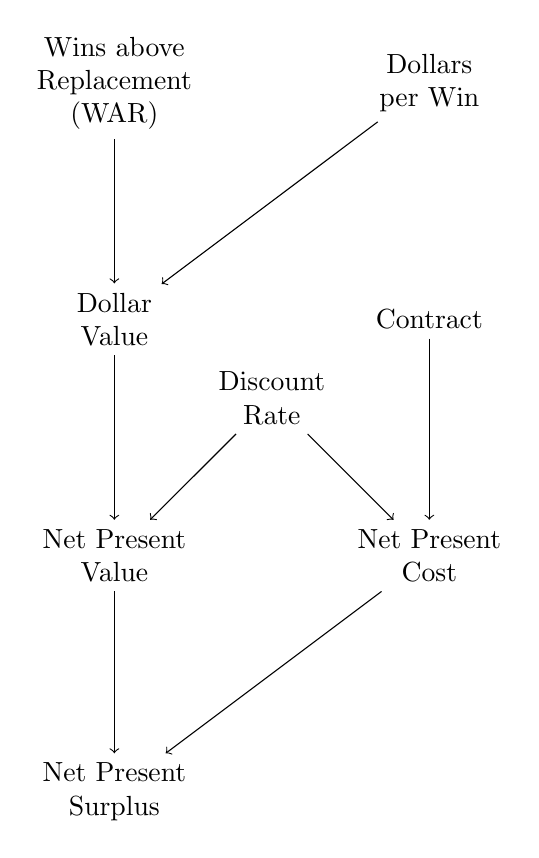
\begin{tikzpicture}
          \node[align=center](war) at (0, 0) {Wins above \\ Replacement \\ (WAR)};
          \node[align=center](dpw) at (4, 0) {Dollars \\ per Win};
          \node[align=center](dollars) at (0, -3) {Dollar \\ Value};
          \node[align=center](contract) at (4, -3) {Contract};
          \node[align=center](discount) at (2, -4) {Discount \\ Rate};
          \node[align=center](npv) at (0, -6) {Net Present \\ Value};
          \node[align=center](npc) at (4, -6) {Net Present \\ Cost};
          \node[align=center](nps) at (0, -9) {Net Present \\ Surplus};
          \draw[->] (war) -- (dollars);
          \draw[->] (dpw) -- (dollars);
          \draw[->] (dollars) -- (npv);
          \draw[->] (contract) -- (npc);
          \draw[->] (discount) -- (npv);
          \draw[->] (discount) -- (npc);
          \draw[->] (npv) -- (nps);
          \draw[->] (npc) -- (nps);
        \end{tikzpicture}
      \end{center}

      \subsubsection{\sc Dollars per Win}

        We value wins based on the cost of paying for wins through free agent contracts, which we observe every off-season. FanGraphs research has shown that it is reasonable to assume free agent contracts are proportional to projected WAR\footnote{\url{https://blogs.fangraphs.com/the-linearity-of-cost-per-win/}} although there is some evidence that higher-WAR players earn more dollars per WAR than average and below-avearge players. To calculate the dollar value of a win above replacement, we can divide free-agent contracts by the player's projected WAR over the length of the contract, with some considerations for inflation over the life of the deal.\footnote{\url{https://baseballprojection.substack.com/p/measuring-the-cost-of-free-agents}}.

        \begin{framed}
          The problem with this framework is that it assumes the same replacement level for all teams, and it assumes that all teams derive the same value from adding a win in free agency. In reality, top teams like the Dodgers have an internal replacement level higher than other teams, and they are also willing to pay more per win than other teams. This explains why top players earn more per WAR. The dollars-per-WAR framework is due for a revamp that acknowledges this dynamic of the competing market forces of teams with different resources and in different situations.
        \end{framed}

      \subsubsection{\sc Deferrals}

        In 2023, Shohei Ohtani and the Los Angeles Dodgers signed a historic 10-year, \$700 million contract with a unique structure. The deal paid Ohtani only \$2 million per year during the playing years 2024--2033, but then the contract pays \$68 million dollars per year from 2034--2043, after Ohtani plays out the contract. This contract structure (paying the player later than the season of their performance) is known as a deferral because the team is deferring payment to the future.

        The key consideration when evaluating contracts with deferrals is discount rate, which is subjective. A dollar today is more valuable than a dollar next year, but the magnitude of this effect depends on your personal preferences. If an aging owner wants to win while they still own the team, they will have a steeper discount rate. If an ownership group thinks they can make strong returns on their financial investments, then they will have a steeper discount rate.

        For the sake of calculating the average annual value (AAV) of contracts for luxury tax purposes, MLB assumes a discount rate of 4.43\% as of the 2022--2026 collective bargaining agreement. Depending on the subjective discount rates of the player and the owner, this may present an opportunity to a structure a deal that is better for both sides. The 2023 Ohtani contract pushed this concept to a new extreme.

      \subsubsection{\sc Player, Team and Mutual Options}

        In 2026, Bo Bichette and the New York Mets signed a 3-year, \$126 million dollar contract that included two player options. After each of the first two years of the contract, Bichette had the option to either to continue the contract or to elect free agency and collect a \$5 million buyout. Bichette had a disappointing year in 2026, accumulating only 1.9 fWAR. He opted into the contract for 2027.

        Player contracts can include three types of options: player options, team options and mutual options. A player option means the player may choose to terminate the contract. A team option means the team may choose to terminate the contract. A mutual option means that either party may choose to terminate the contract. Generally, contract termination includes a buyout payment from the team to the player. Typically, a player will choose to opt out if their market value exceeds the remainder of the contract, and a team will choose to opt out if the player's market value is below the remainder of the contract. Mutual options are an curious phenomenon that almost always result in one side or the other opting out.

        Player options make the contract more appealing to the player, and team options make the contract more appealing to the team. To value contracts with options, teams use simulations to model the probably of the option being exercised or the contract being terminated, as well as the conditional expectation of the surplus value of the contract given that it is exercised. This requires projections that quantify uncertainty over the player's talent development.

        Team options are another reason that players under ``team control'' are so valuable to clubs. Before a player accumulates three years of major league service time, their salary is effectively the league minimum in the next three years before the player accumulates six years of major league service time, their salary is determined via arbitration, below the market rate in free agency. Throughout all of these years, the club has a team option every single year, capturing the upside if the player breaks out without any of the downside if the player doesn't pan out. Again, simulating the player's career development with projections that have uncertainty quantification allow teams to price these contracts appropriately.

\end{document}